% Make nice A4 pages for print:
%\usepackage{pgfpages}
%\pgfpagesuselayout{resize to}[a4paper,border shrink=5mm,landscape]

\beamertemplatenavigationsymbolsempty

\setbeamertemplate{bibliography item}[text]

\usepackage[type={CC},modifier={by-sa},version={4.0}]{doclicense}

\usepackage[utf8]{inputenc}
\usepackage{hyperref}
\usepackage{breakurl}
\usepackage{graphicx}
\usepackage{pgfplots}
\usepackage{pgf}
\usepackage{tikz}
\usetikzlibrary{positioning}
\usetikzlibrary{arrows}
\usetikzlibrary{decorations.markings}
\usetikzlibrary{calc}
\usetikzlibrary{matrix}
\usetikzlibrary{shapes}
\usetikzlibrary{decorations.pathmorphing}
\usetikzlibrary{fit}
\usetikzlibrary{backgrounds}
\usetikzlibrary{plotmarks}
\usepackage{stmaryrd}
\usepackage{listings}
\usepackage{pdflscape}
\usepackage{perpage}
\usepackage{appendixnumberbeamer}

%\usepackage[thmmarks,amsmath,amsthm]{ntheorem} % already included in beamer
\usepackage{thm-restate}

\usepackage[sort&compress,numbers]{natbib}  % to be have \citet, \citeauthor, \citeyear

\MakePerPage{footnote}

\tikzstyle{o}=[r,ppBlue]
\tikzstyle{r}=[thick,rectangle,align=center]
\tikzstyle{t}=[r,ppTrans] %,font=\bfseries]
\tikzstyle{dd}=[densely dashed]
\tikzstyle{n}=[r,ppBlue]
\tikzstyle{p}=[r,ppRed]
\tikzstyle{ppRed}  =[draw=red,  fill=  red!20]
\tikzstyle{ppBlue} =[draw=blue, fill= blue!20]
\tikzstyle{ppGreen}=[draw=green,fill=green!20]
\tikzstyle{ppTrans}=[draw=none, fill=none]

\usetheme{Warsaw}

\useoutertheme[subsection=true]{smoothbars}
%\useoutertheme[subsection=false]{miniframes}

\definecolor{bblue}{HTML}{D7DF01}	% yellow-ish actually, for better black/white printing
\definecolor{rred}{HTML}{C0504D}
\definecolor{ggreen}{HTML}{9BBB59}
\definecolor{ppurple}{HTML}{9F4C7C}
\definecolor{lightgray}{rgb}{0.3,0.3,0.3}
\definecolor{lightergray}{rgb}{0.9,0.9,0.9}
\definecolor{UniBlue}{RGB}{83,121,170}

\DeclareTextFontCommand\textintro{\normalfont\bfseries\itshape} % nice!
\newcommand{\intro}[2][]
{%
	\textintro{#2}%
}
\newcommand{\empha}[2][]
{%
	\emph{#2}%
}

%\theoremstyle{plain}
\newcounter{reqcounter}
\newtheorem{requirement}[reqcounter]{Requirement}

%setbeamercolor{structure}{fg=violet}

\makeatletter
\def\th@task{%
    \normalfont % body font
    \setbeamercolor{block title example}{bg=orange,fg=white}
    \setbeamercolor{block body example}{bg=orange!20,fg=black}
    \def\inserttheoremblockenv{exampleblock}
  }
\makeatother

\theoremstyle{task}
\newtheorem{task}{Task}

\newenvironment{assignment}%
{%\setbeamercolor{background canvas}{bg=violet}%
%\setbeamercolor{structure}{fg=cyan!90!black}%
 \setbeamercolor{frametitle}{bg=orange,fg=white}
\begin{frame}}%
{\end{frame}}%

\AtBeginSection[]{
  \begin{frame}
  \vfill
  \centering
  \begin{beamercolorbox}[sep=8pt,center,shadow=true,rounded=true]{title}
    \usebeamerfont{title}\insertsectionhead\par%
  \end{beamercolorbox}
  \tableofcontents
  \vfill
  \end{frame}
}




\pgfplotsset{compat=1.14}
\author{Markus Raab}


\date{13.03.2019}

\begin{document}

\renewcommand{\enquote}[1]{\emph{``#1''}} % Cannot be done earlier

%%%%%%%%%%%%%%%%%%%%%%%%%%%%%%%
\begin{frame}
	\titlepage
	\doclicenseThis
\end{frame}

%%%%%%%%%%%%%%%%%%%%%%%%%%%%%%%%%%%%%%%%%% 
\section{Background}
{
\shadowcolor{black}
\shadowoffset{0.5pt}
\usebackgroundtemplate{\includegraphics[width=\paperwidth]{pics/clouds.jpg}}%
\begin{frame}
	\frametitle{\shadowtext{Misconfiguration}}
	\begin{itemize}
		\item   \textcolor{white}{\shadowtext{\empha[misconfiguration]{misconfigurations}~\cite{yin2011empirical,su2007autobash,attariyan2010automating,xu2015systems} are a major cause}}\\
			\textcolor{white}{\shadowtext{of system failures~\cite{wool2004quantitative,oppenheimer2003internet,pertet2005causes}}}
		\item   \textcolor{white}{\shadowtext{much time needed to fix misconfigurations~\cite{rabkin2011static,oppenheimer2003internet,yin2011empirical,mahajan2002bgp}}}
		\item   \textcolor{white}{\shadowtext{configuration is a user interface for both developers}}\\
			\textcolor{white}{\shadowtext{and system administrators}}
	\end{itemize}
\end{frame}
}
\begin{frame}
	\frametitle{No-Futz}
	\begin{itemize}
		\item \citet{holland2001nofutz}~defined \empha{futzing} to denote \enquote{tinkering or fiddling experimentally with something.}
		\item With \intro[no-futz computing]{no-futz computing} \citet{holland2001nofutz} mean \enquote{that futzing should be allowed, but should never be required.}
		\item currently configuration is error-prone and under-specified, \empha{futzing} is often required
	\end{itemize}
\end{frame}

\section{Elektra}

\begin{frame}
	\frametitle{SpecElektra}

	\fontsize{18}{0}\selectfont
	\ExecuteMetaData[../book/approach.tex]{definition-spec}
\end{frame}

\begin{frame}
	\frametitle{Recapitulation (Requirements of SpecElektra)}

	\pause
	\begin{itemize}
	\item formal and informal
	\item should strive for completeness
	\item should be extensible
	\item should be external to application
	\item open for introspection (for tooling)
	\item should talk to users
	\item should allow generation of artefacts
	\end{itemize}
\end{frame}




\begin{frame}[fragile]
	\frametitle{KeySet Generation}
	\begin{alertblock}{Question}
	Idea: What if the configuration file format grammar describes source code?
	\end{alertblock}
	\pause

	\begin{grammar}
	<KeySet> ::= \lq ksNew'\WhiteSpace(' \{ <Key> \lq , \LineBreak'  \}  \{ \lq\WhiteSpace' \} \lq KS\_END);'

	<Key> ::= \lq keyNew \WhiteSpace ('' ' <key name> \lq ''  , \LineBreak' [ <Value> ] <properties> \lq KEY_END)'

	<Value> ::=  \{ \lq\WhiteSpace' \} \lq KEY\_VALUE, \WhiteSpace '' ' <configuration value> \lq ''  , \LineBreak'

	<properties> ::= \{ \{ \lq\WhiteSpace' \} <property> \lq , \LineBreak' \}

	<property> ::=  \lq KEY\_META, \WhiteSpace " ' <property name> \lq "  , \WhiteSpace " ' <property value> \lq " '
	\end{grammar}
\end{frame}

\begin{frame}[fragile]
	\frametitle{Example}
	\begin{example}
	Given the key ^spec:/slapd/threads/listener^, with the configuration value ^4^ and the property $\property{default} \mapsto 1$, \elektra{Gen} emits:

	\begin{code}[gobble=4,language=Cpp]
	ksNew (keyNew ("spec:/slapd/threads/listener",
		       KEY_VALUE, "4",
		       KEY_META, "default", "1",
		       KEY_END),
	       KS_END);
	\end{code}
	\vspace{-1em}
	\end{example}

	\pause
	\begin{alertblock}{Finding}
	We have source code representing the settings.
	And if we instantiate it, we have a data structure representing the settings.
	Plugins emitting such ``configuration files'' are code generators.
	\end{alertblock}
\end{frame}

\begin{frame}[fragile]
	\frametitle{Implementation Strategies}

	\begin{itemize}
	\item Using ^print^ (only for very small generators)
	\item Using generative grammars
	\begin{code}[gobble=4,language=Cpp]
	query = '{' >> *(pair) > '}';
	pair = '{' >> key_name > '=' >> key_value >>
	       *('{' >> metakey_name > '=' >> metakey_value > '}')
	       > '}';
	\end{code}
	\item Using template languages (RubyERB, Cheetah, Mustache)
	\begin{code}[gobble=4,language=Python,basicstyle=\ttfamily\tiny,numberstyle=\ttfamily\tiny\color{blue}]
	@for n in hierarchy.name.split('/')[1:-1]
	namespace $support.nsnpretty($n)
	{
	class ${hierarchy.prettyclassname(support)}
	{
	typedef $support.typeof($hierarchy.info) type;
	@if $support.typeof($hierarchy.info) != "kdb::none_t"
	static type get(kdb::KeySet &ks, kdb::Key const& spec)
	{
		type value $support.valof($hierarchy.info)
		Key found(ckdb::ksLookup(ks.getKeySet(), *spec,
					ckdb::elektraLookupOptions::KDB_O_SPEC));
		return found.get<$support.typeof($hierarchy.info)>();
	}
	\end{code}
	\end{itemize}
\end{frame}

\begin{frame}
	\frametitle{Possible Properties}
	For example, SpecElektra has following properties:
	\begin{description}
	\item[type] represents the type to be used in the emitted source code.
	\item[opt] is used for short command-line options to be copied to the namespace \namespace{proc}.
	\item[opt/long] is used for long command-line options, which differ from short command-line options by supporting strings and not only characters.
	\item[restrict/write] yields compilation errors when developers assign a value to a contextual value within the program.
	\item[default] enables us to start the application even if the backend does not work.
	\end{description}
\end{frame}

\begin{frame}[fragile]
	With the specification:
	\par
	\begin{code}[gobble=4]
	[foo/bar]
	  default:=Hello
	  type:=string
	  opt:=b
	  restrict/write:=1
	\end{code}
	\par
	\elektra{Gen} gives the user read-only access to the object ^env.foo.bar^:
	\par
	\begin{code}[language=Cpp]
	std::cout << env.foo.bar;
	env.foo.bar = "Other world"; // comp. error
	\end{code}
	\par
	\small
	\pause
	Line~1 prints the configuration value of ^/foo/bar^ or ^"Hello"^ (without quotes) by default.
	When invoking the application with ^application -b "This world"^, the application would print ^"This world"^ (without quotes).
	Line~2 leads to a compilation error because of the property \property{restrict/write}.
\end{frame}



% hack: needed to render graphics properly
\begin{frame}<0>[noframenumbering]
	\begin{columns}[c]
	\begin{column}{7cm}
	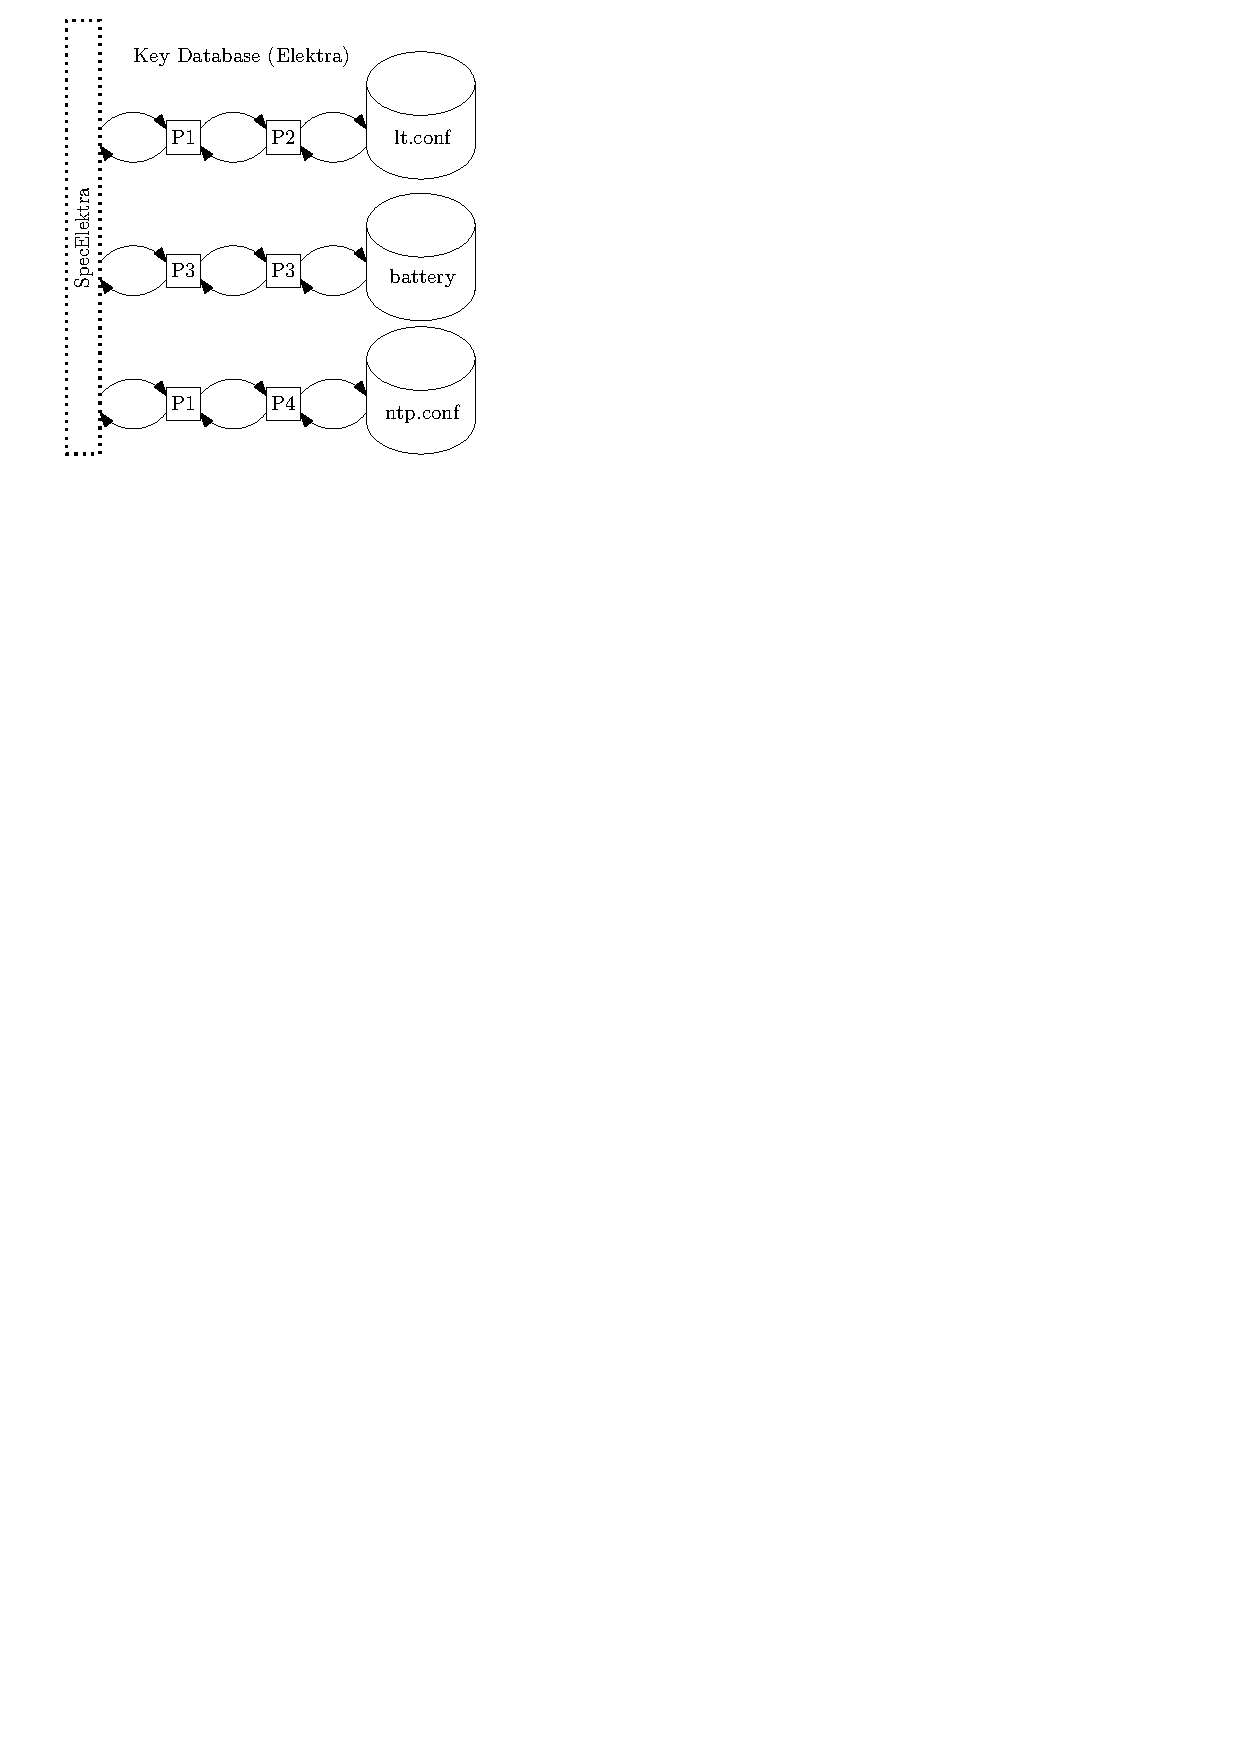
\includegraphics[scale=0.8]{horizontalmodularity}
	\end{column}
	\begin{column}{4cm}
	Cylinders are configuration files, P? are plugins~\cite{raab2016improving}.

	Key ideas:
	\begin{itemize}
	\item all work is done by plugins
	\item central data structure implements semantics
	\end{itemize}
	\end{column}
	\end{columns}
\end{frame}

\begin{frame}
	\begin{columns}[c]
	\begin{column}{7cm}
	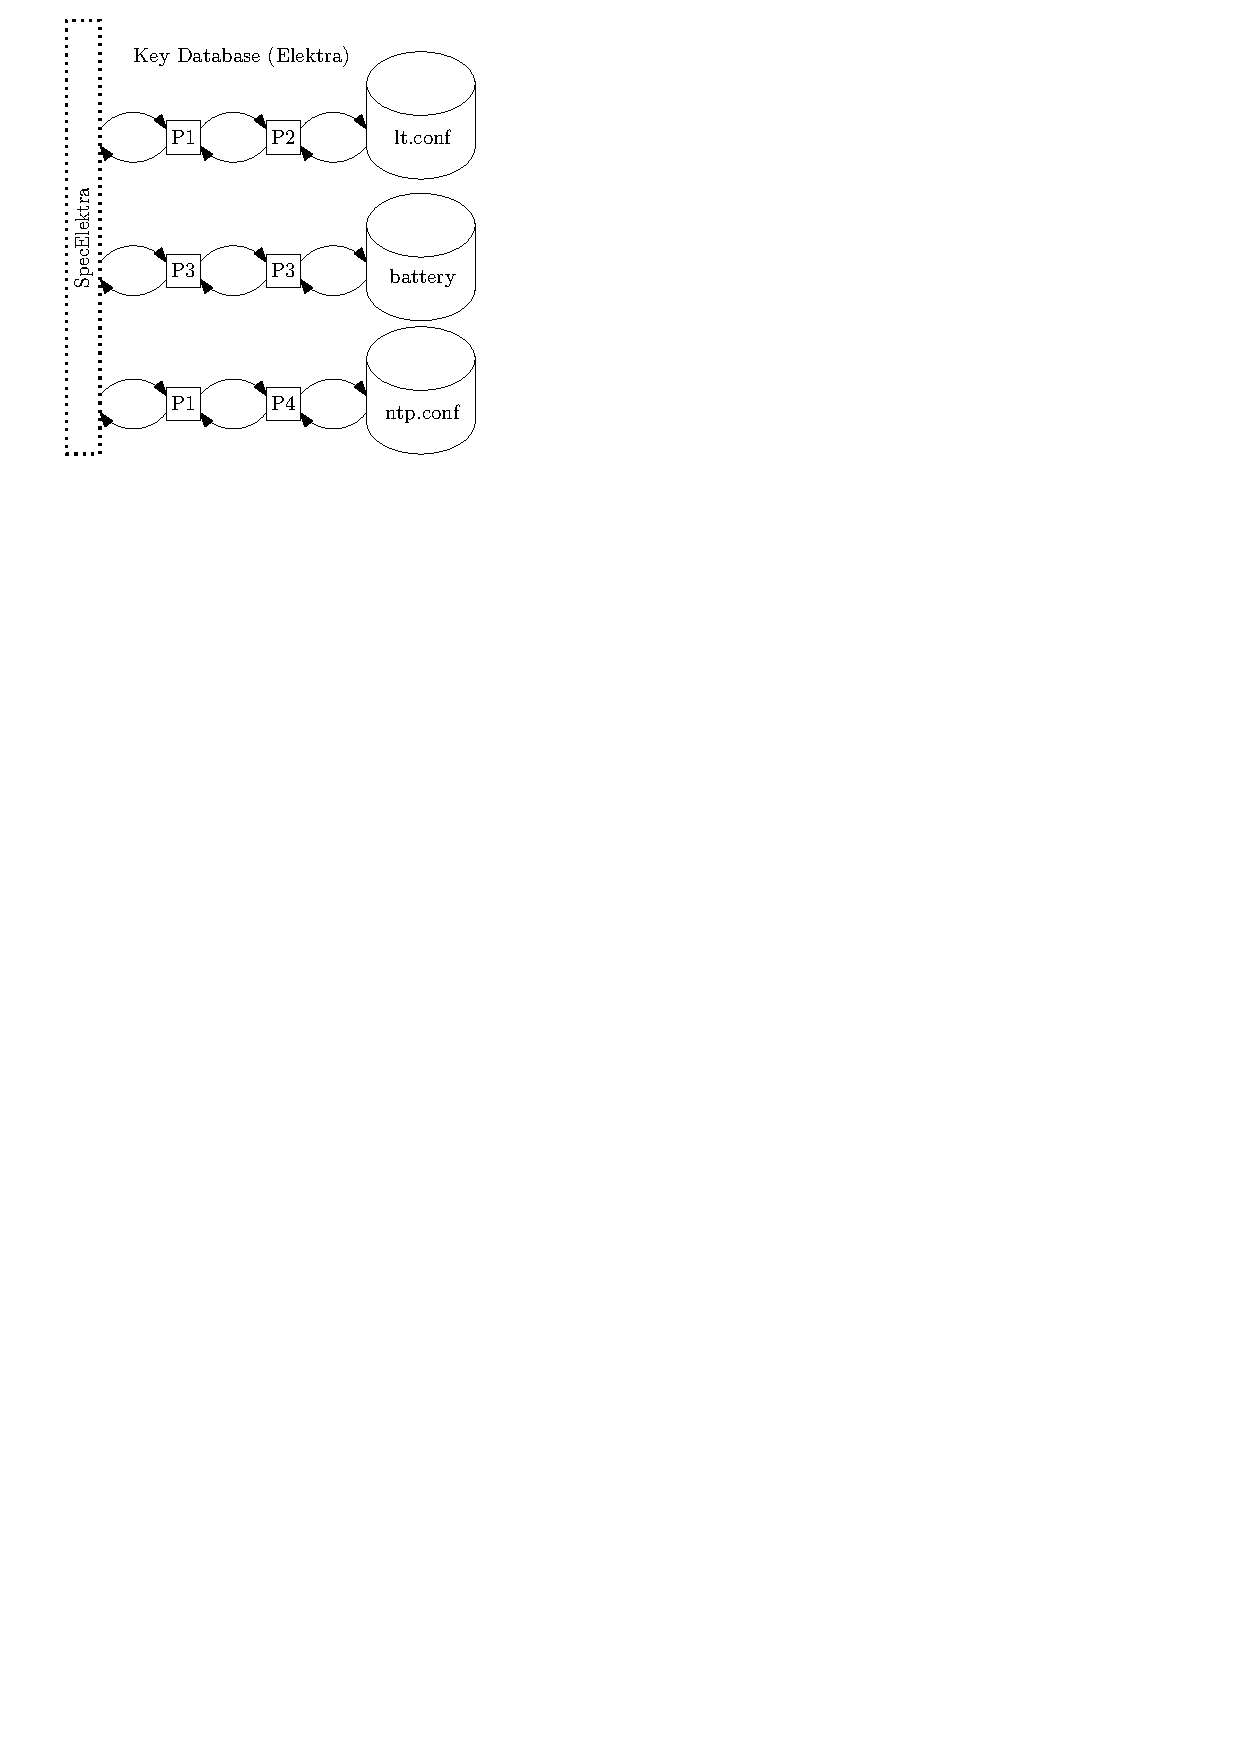
\includegraphics[scale=0.8]{horizontalmodularity}
	\end{column}
	\begin{column}{4cm}
	Cylinders are configuration files, P? are plugins~\cite{raab2016improving}.

	Key ideas:
	\begin{itemize}
	\item all work is done by plugins
	\item central data structure implements semantics
	\end{itemize}
	\end{column}
	\end{columns}
\end{frame}

\begin{frame}
	\frametitle{KeySet}

	The common data structure between plugins:
	\vspace{1cm}

	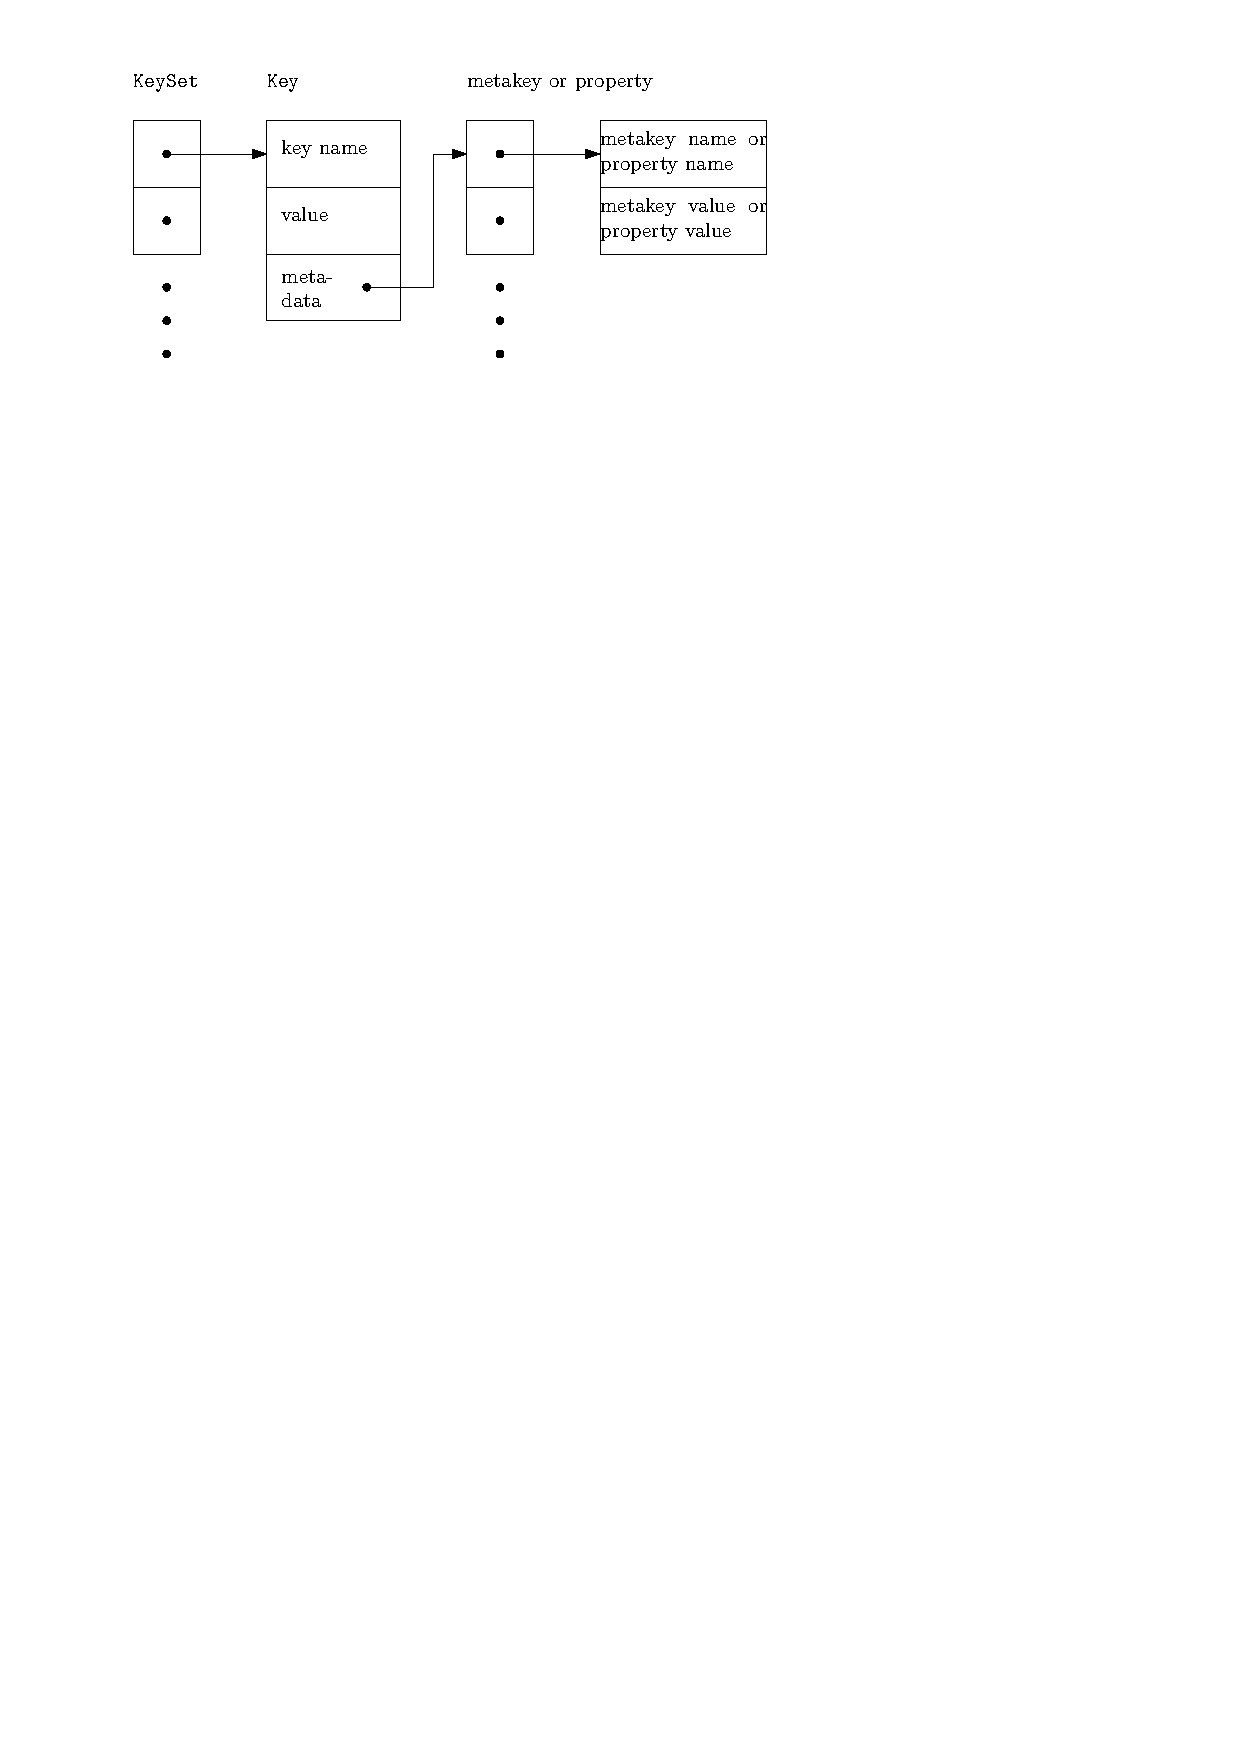
\includegraphics{keyset}
\end{frame}

\begin{assignment}
	\begin{task}
	Is meta-data separated from or included in the data structure?
	\end{task}
\end{assignment}

\subsection{Metalevels}

\begin{frame}
	\frametitle{Metalevels}
	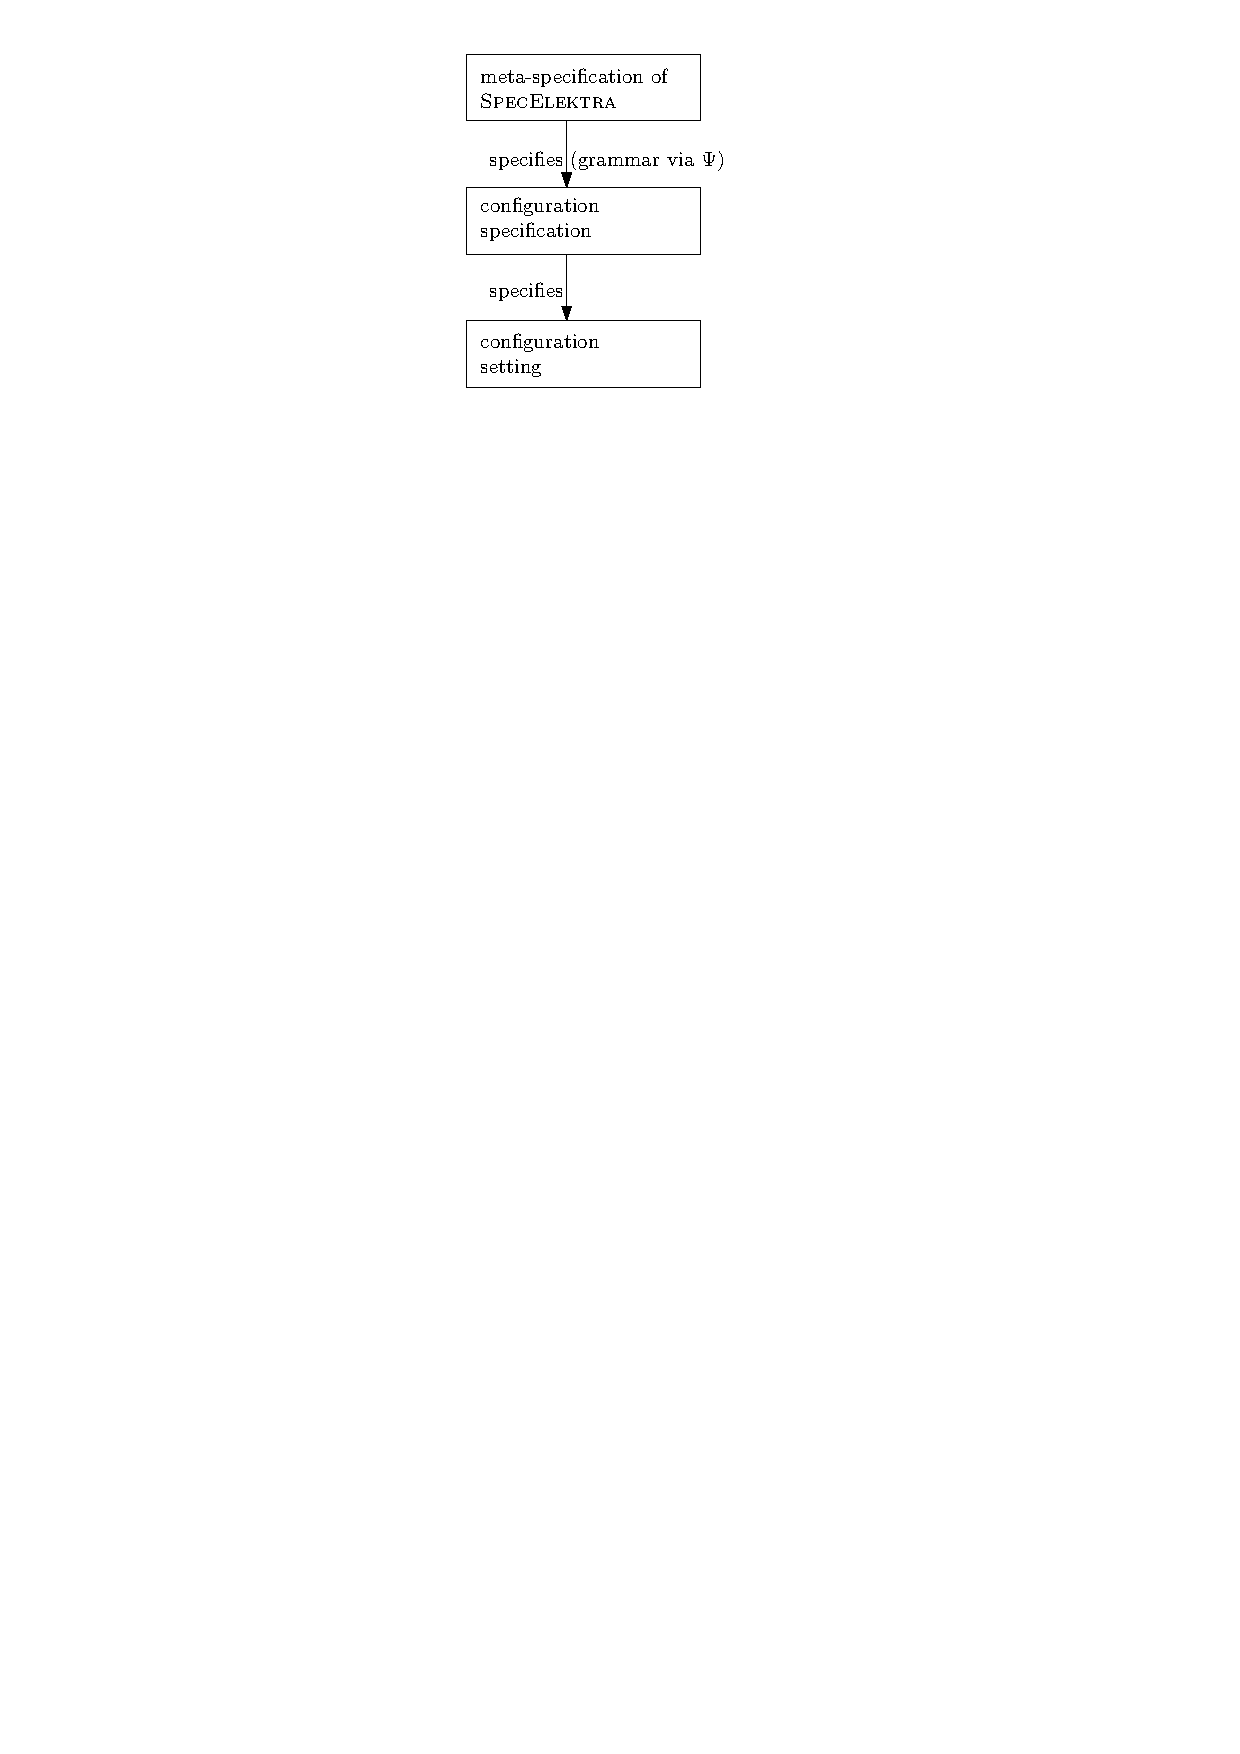
\includegraphics{metalevels}

	We will now walk through metalevels bottom-up.
\end{frame}

\begin{frame}[fragile]
	\frametitle{Configuration Settings}

	A configuration file may look like:

	\begin{code}[language=CfgElektra]
	a=5
	b=10
	c=15
	\end{code}

	We apply these configuration settings imperatively using:

	\begin{code}[language=bash]
	kdb set /a 5
	kdb set /b 10
	kdb set /c 15
	\end{code}

	And we list them with \lstinline[language=bash,morekeywords={ls},showspaces=no]^kdb ls /^.
\end{frame}

\begin{frame}[fragile]
	\frametitle{Specifications}
	For specifications such as:

	\begin{code}
	[slapd/threads/listener]
	  check/range:=1,2,4,8,16
	  default:=1
	\end{code}

	We apply the specifications imperatively using:

	\begin{code}[language=bash,morekeywords={setmeta}]
	kdb setmeta /slapd/threads/listener\
		check/range 1,2,4,8,16
	kdb setmeta /slapd/threads/listener\
	       	default 1
	\end{code}

	(automatically uses ^spec^ namespace)
\end{frame}

\begin{frame}[fragile]
	\frametitle{Meta-Specifications}
	For meta-specifications such as:

	\small
	\begin{code}
	[visibility]
	type:=enum critical important user\
	      advanced developer debug disabled
	description:=Who should see this\
	     configuration setting?
	\end{code}

	We apply the meta-specifications imperatively using:

	\begin{code}[language=bash,morekeywords={setmeta}]
	kdb setmeta /elektra/meta/\
		visibility type enum ...
	kdb setmeta /elektra/meta/\
		visibility description "Who ...
	\end{code}

	(see ^doc/METADATA.ini^, disclaimer: 1.0 not yet released)
\end{frame}

\subsection{Conclusions}

\begin{frame}
	\frametitle{Introspection}
	\begin{itemize}[<+->]
	\item unified get/set access to (meta*)-key/values
	\item access via applications, CLI, GUI, web-UI, ...
	\item GUI, web-UI can semantically interpret metadata
	\item access via any programming language
	\item access via any configuration management system
	\end{itemize}
\end{frame}

\begin{frame}
	\frametitle{Users of Elektra}
	\begin{itemize}[<+->]
	\item Embedded systems
	\begin{itemize}
	\item OpenWRT (distribution)
	\item Broadcom (blue-ray devices)
	\item Kapsch (cameras)
	\item Toshiba (TVs)
	\end{itemize}
	\item Server
	\begin{itemize}
	\item Allianz (insurance)
	\item TU Wien
	\item puppet-libelektra
	\item Other Universities
	\end{itemize}
	\item Desktop
	\begin{itemize}
	\item Oyranos
	\item LCDproc (in progress)
	\item KDE
	\end{itemize}
	\end{itemize}
\end{frame}

%%%%%%%%%%%%%%%%%%%%%%%%%%%%%%%%%%%%%%%%%% 
\section{Configuration Management}

\begin{frame}[fragile]
	Key/value access in Chef:

	\begin{code}[morekeywords={kdbset,do,action,value,end},gobble=4]
	kdbset 'system/sw/samba/global/workgroup' do
		value 'MY_WORKGROUP'
		action :create
	end
	\end{code}
\end{frame}

\begin{frame}[fragile]
	Key/value access in Ansible:

	\begin{code}[morekeywords={name,connection,key,value,elektra,mountpoint,file,plugins,hosts,tasks},gobble=4]
	- name: setup samba
	  connection: local
	  hosts: localhost
	  tasks:
	  - name: set workgroup
	    elektra:
	      mountpoint: system/sw/samba
	      file: /etc/samba/smb.conf
	      plugins: ini
	    elektra:
	      key: 'system/sw/samba/global/workgroup'
	      value: 'MY_WORKGROUP'
	\end{code}
\end{frame}

\begin{frame}[fragile]
	Key/value access in puppet-libelektra:

	\begin{code}[morekeywords={kdbkey,kdbmount,ensure,value},gobble=4]
	kdbmount {'system/sw/samba':
		ensure => 'present',
		file => '/etc/samba/smb.conf',
		plugins => 'ini'
	}
	kdbkey {'system/sw/samba/global/workgroup':
		ensure => 'present',
		value => 'MY_WORKGROUP'
	}
	kdbkey {'system/sw/samba/global/log level':
		ensure => 'absent'
	}
	\end{code}

	Uniqueness of keys is essential.
	Ideally, applications already mount their configuration at installation.
\end{frame}


\begin{frame}[fragile]
	Key/value specifications in puppet-libelektra:

	\begin{code}[morekeywords={kdbkey,ensure,value},gobble=4]
	kdbkey {'system/sw/samba/global/log level':
		ensure => 'present',
		value => 'MY_WORKGROUP',
		check => {
			'type' => 'short',
			'range' => '0-10',
			'default' => '1',
			'description' => 'Sets the amount of log/
				debug messages that are sent to the
				log file. 0 is none, 3 is consider-
				able.'
	}
	\end{code}

	Ideally, applications already specify their settings.
\end{frame}


%%%%%%%%%%%%%%%%%%%%%%%%%%%%%%%%%%%%%%%%%%%%%%%%%%%%
\section{Problems in Flexibility}

\subsection{Feature Interaction}

\subsection{Integration of Operators}

\begin{frame}
	\frametitle{Key-Value}
A key-value pair is the simplest generic data structure~\cite{strang2004context}.
While all these formats above have many differences, all of them represent configuration settings as \intro[key-value pair]{key-value pairs}~\cite{jin2014configurations,rabkin2011static,xu2013blame,lathia2013open}.
\\[1cm]

For configuration as program you need to execute them first.
\end{frame}


\section{Conclusion}

\begin{frame}
	\frametitle{Conclusion}
	\begin{itemize}
	\item make simple configuration management tasks simple
	\item operators not always combinable
	\item plugin development needs careful consideration of interactions
	\end{itemize}
\end{frame}



%%%%%%%%%%%%%%%%%%%%%%%%%%%%%%%%%%%%%%%%%% 
\nocite{raab2017introducing}

\appendix

\begin{frame}[allowframebreaks]
	\bibliographystyle{plainnat}
	\bibliography{../shared/elektra.bib}
\end{frame}

\end{document}


